\section{Detection des Cibles et Courbe ROC}
 
\subsection{\textit{True Positive Rate} (TPR) et \textit{False Positive Rate} (FPR)}

L'axe des abscisses dans la courbe ROC représente le FPR , également appelé taux de faux positifs. C'est la proportion d'échantillons de la classe négative qui sont incorrectement classés comme positifs par le modèle. Mathématiquement, le FPR est défini par l'équation \ref{eq:FPR}.

\begin{equation}
    FPR = \frac{\text{False Positives}}{\text{False Positives} + \text{True Negatives}}
    \label{eq:FPR}
\end{equation}


L'axe des ordonnées dans la courbe ROC représente le TPR  ou la sensibilité. Il s'agit de la proportion d'échantillons de la classe positive correctement classés comme positifs par le modèle. Le TPR est défini par l'quation \ref{eq:TPR}.

\begin{equation}
    TPR = \frac{\text{True Positives}}{\text{True Positives} + \text{False Negatives}}
    \label{eq:TPR}
\end{equation}

Maintenant, le lien avec la fonction \texttt{detect\_targets} est le suivant : la fonction génère une matrice booléenne (\texttt{binary\_map}) en appliquant un seuil à la RDM. Cette matrice est utilisée pour calculer le FPR et le TPR dans le contexte de la courbe ROC. Les vrais positifs et les faux positifs sont déterminés en comparant la résultante avec les véritables états de présence de cibles. Mathématiquement, la fonction \texttt{detect\_targets} peut être réprésenté:
\[
binary\_map=\begin{cases} 
True & \text{si } \text{{rdm > thresholds}} \\
False & \text{sinon}
\end{cases}
\]
\subsection{Courbe ROC }

La courbe ROC  est un outil essentiel pour évaluer la performance du radar \textit{FMCW} dans différents scénarios de bruit. Cette courbe illustre graphiquement la relation entre les taux de faux positifs (FPR) et de vrais positifs (TPR) en fonction des seuils de détection. Elle est calculée en utilisant la RDM sans bruit comme référence et en appliquant des seuils aux RDM avec bruit et ce pour différents niveaux de bruits.

Le graphe ROC, basé sur différentes valeurs de SNR, est présenté dans la figure \ref{fig:roc}. Il démontre la performance du radar pour chaque scénario de bruit, indiquant le compromis entre le TPR et le FPR. La ligne en pointillés représente le résultat attendu pour un modèle aléatoire.

\begin{figure}[H]
    \centering
    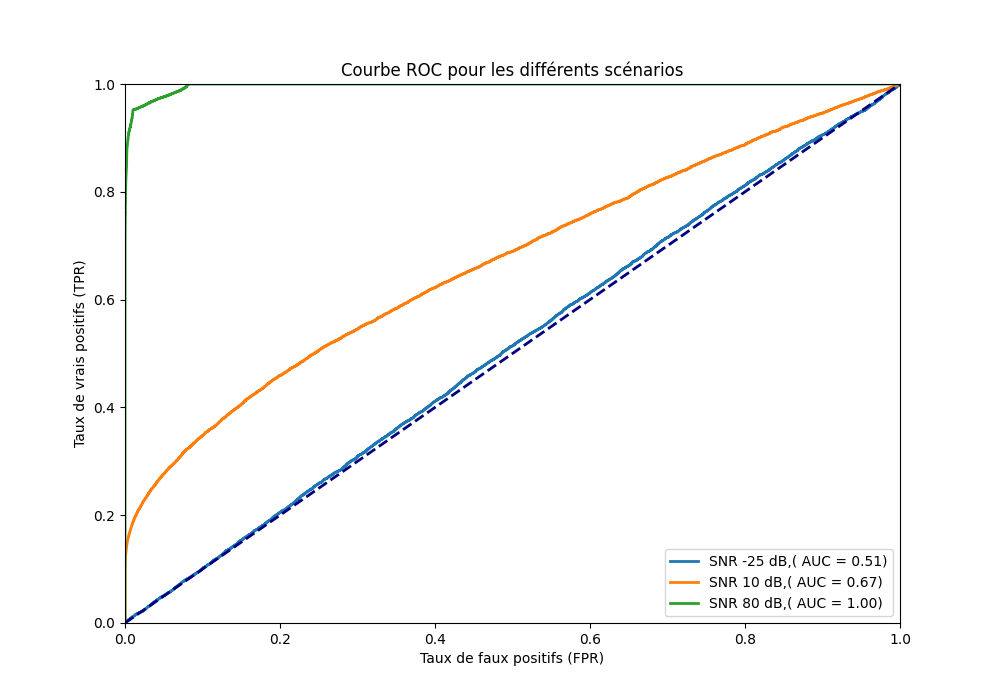
\includegraphics[width=0.8 \textwidth]{Pictures/ROC_SST_P.png}
    \caption{Courbe ROC pour les différents niveaux de bruits.}
    \label{fig:roc}
\end{figure}

L'aire sous la courbe (AUC) est calculée pour chaque valeur de SNR et est indiquée dans la légende du graphe. Une AUC proche de 1 indique une excellente performance, tandis qu'une valeur proche de 0.5 suggère une performance aléatoire.\\
\textbf{Discussion des valeurs des SNR}\\
Il est intéressant de voir que des valeurs de SNR plus élevées conduisent généralement à des AUC plus grandes, indiquant une meilleure capacité du radar à discriminer entre les cibles réelles et le bruit. Cela met en évidence l'importance des valeurs de SNR dans l'efficacité du radar en conditions réelles.
